\begin{subfigure}{0.4\textwidth}
		\centering
		\tdplotsetmaincoords{70}{110}
		\tdplotsetrotatedcoords{0}{0}{0}
		\begin{tikzpicture}[scale = 0.45,tdplot_rotated_coords]
		
		\coordinate (p1b) at (0,1,5);
		\coordinate (p2b) at (0,3,5);
		\coordinate (p3b) at (0,6,3);
		\coordinate (p4b) at (0,6,-2);
		\coordinate (p5b) at (0,1,-2);
		\coordinate (p1f) at (5,1,5);
		\coordinate (p2f) at (5,3,5);
		\coordinate (p3f) at (5,6,3);
		\coordinate (p4f) at (5,6,-2);
		\coordinate (p5f) at (5,1,-2);
		
		\draw (p1b) -- (p2b) -- (p3b) -- (p4b);% -- (p5b) -- cycle;
		\draw[fill=black!10] (p1f) -- (p2f) -- (p3f) -- (p4f) -- (p5f) -- cycle;
		\draw (p1f) -- (p1b);
		\draw (p2f) -- (p2b);
		\draw (p3f) -- (p3b);
		\draw (p4f) -- (p4b);
		
		\draw[->,thick] (5,3.5,0.5) -- (5,3.5,2.5);
		\node (M1) at (5,4,1.5) {\textbf{M}};
		\end{tikzpicture}
		\caption{}
		\label{fig:p13dpolyhedron}
	\end{subfigure}
	
	\vspace{20pt}
	
	\begin{subfigure}{0.4\textwidth}
		\centering
		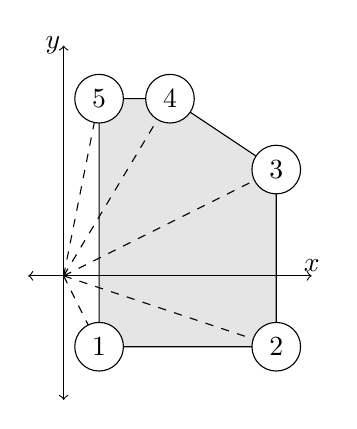
\begin{tikzpicture}[scale=0.45]
		\coordinate (origin) at (0,0);
		\coordinate (p5) at (1,5);
		\coordinate (p4) at (3,5);
		\coordinate (p3) at (6,3);
		\coordinate (p2) at (6,-2);
		\coordinate (p1) at (1,-2);
		
		\filldraw[fill = black!10] (p1) -- (p2) -- (p3) -- (p4) -- (p5) -- cycle;
		
		\draw[dashed] (origin) node {} -- (p1) node[circle,fill=white,draw,solid] {1};
		\draw[dashed] (origin) node {} -- (p2) node[circle,fill=white,draw,solid] {2};
		\draw[dashed] (origin) node {} -- (p3) node[circle,fill=white,draw,solid] {3};
		\draw[dashed] (origin) node {} -- (p4) node[circle,fill=white,draw,solid] {4};
		\draw[dashed] (origin) node {} -- (p5) node[circle,fill=white,draw,solid] {5};
		
		\node (x) at (7,0.3){\(x\)};
		\node (y) at (-0.3,6.5){\(y\)};
		
		\draw [<->] (-1,0) -- (7,0);
		\draw [<->] (0,-3.5) -- (0,6.5);
		\end{tikzpicture}
		\caption{}
		\label{fig:p1polygondecomposition}
	\end{subfigure}
	~
	\begin{subfigure}{0.4\textwidth}
		\centering
		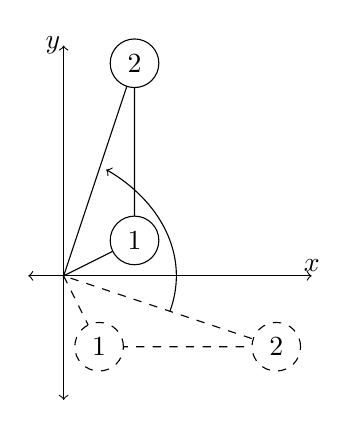
\begin{tikzpicture}[scale=0.45]
		\coordinate (origin) at (0,0);
		\coordinate (p2) at (2,1);
		\coordinate (p1) at (2,6);
		
		\draw[solid] (p1) -- (origin) -- (p2) -- cycle;
		\path (p1) node[circle,fill=white,draw,solid] {2} -- (p2) node[circle,fill=white,draw,solid] {1};
		
		\draw[dashed] (0,0) -- (1,-2) -- (6,-2) -- cycle;
		\path (6,-2) node[circle,fill=white,draw,dashed] {2} -- (1,-2) node[circle,fill=white,draw,dashed] {1};
		
		\node (x) at (7,0.3){\(x\)};
		\node (y) at (-0.3,6.5){\(y\)};
		
		\draw [<->] (-1,0) -- (7,0);
		\draw [<->] (0,-3.5) -- (0,6.5);
		
		\draw[<-] (1.2,3) to [out=-30,in=70] (3,-1.0);
		\end{tikzpicture}
		\caption{}
		\label{fig:p1makingtriangles}
	\end{subfigure}